% Latex template for submission to the 16th International Meeting on Fully 3D Image Reconstruction 
% in Radiology and Nuclear Medicine (Fully3D 2021)
%
% Author: G.Schramm
% Date:   Oct 2020
%
% In case you encouter problems, you can raise a github issue here:
% https://github.com/gschramm/fully3d_2021_templates/issues
%
% 
% To build this document, we recommend to use latexmk via:
% ```latexmk -pdf fully3d_template.tex```
% Building in the online editor overleaf also works.

\documentclass[11pt,twocolumn,twoside]{article}
\usepackage{fully3d}

%%%%%% add your extra packages here (if needed)                                       %%%%%
%%%%%% before, have a look which packages are already imported by the fully3d package %%%%%

\usepackage{amssymb}
\usepackage{algorithmicx}
\usepackage{algpseudocode}

%\newtheorem{rem}{Remark}

% define float env for algorithm
\usepackage{float}
\floatstyle{ruled}
\newfloat{algorithm}{h}{loa}
\floatname{algorithm}{Algorithm}

%%%%% add your bibtex file that contains the bibtex entries here %%%%%
%%%%% please include DOIs in the bibtex entries if possible      %%%%%
\addbibresource{fully3d_2021.bib}

% custom definitions
\DeclareMathOperator{\proj}{proj}
\DeclareMathOperator{\prox}{prox}
\DeclareMathOperator*{\argmin}{arg\,min}

\begin{document}


%-------------------------------------------------------------------------------------------
%%%%% add your title here %%%%%
\title{Fast and memory-efficient reconstruction of sparse TOF PET data with non-smooth priors} 

%%%%% add authors and affiliations here %%%%%
\author[1]{Georg~Schramm}
\author[2]{Martin~Holler}

\affil[1]{Department of Imaging and Pathology, Division of Nuclear Medicine,
          KU Leuven, Belgium}

\affil[2]{Institute of Mathematics and Scientific Computing, 
          University of Graz, Austria}

%%%%% don't change these 2 lines %%%%%
\maketitle
\thispagestyle{fancy}



%-------------------------------------------------------------------------------------------
%%%%% add your summary (abstract) here               %%%%%%
%%%%% use footnotesize for this section              %%%%%%
%%%%% please stick to the customabstract environment %%%%%% 


\begin{customabstract}
In this work, we propose and analyze a modification of the stochastic primal-dual hybrid gradient
(SPDHG) algorithm which substantially reduces its memory requirements 
for reconstruction of sparse time-of-flight (TOF) PET data with non-smooth priors.
Moreover, we study the influence of the ratio of the primal and dual step sizes 
on the convergence of SPDHG.
The performance of the optimization algorithm is investigated based on simulated 2D TOF
data using a brain-like software phantom.
We find that the memory requirement of SPDHG for sparse TOF PET data can be
substantially reduced by a better initialization without noticeable losses in the convergence speed.
Moreover, a careful choice of the ratio of the primal and dual step sizes, 
depending on the magnitude of the image to be reconstructed, is crucial to obtain fast convergence.
\end{customabstract}


%-------------------------------------------------------------------------------------------
%%%%% main text %%%%%    
\section{Introduction}

Due to limitations in acquisition time, injectable dose and scanner sensitivity,
acquired data in positron emission tomography (PET) suffer from high levels of
Poisson noise that is transferred into the reconstructed image, necessitating
noise suppression during or post reconstruction.
One possible way of noise suppression is the maximum a posteriori approach
where a smoothing prior is added next to the data fidelity term (the negative
Poisson loglikelihood) in the cost function optimized in iterative image 
reconstruction.
Unfortunately, many advanced smoothing priors such as e.g. Total Variation (TV) \cite{Rudin1992},
Total Generalized Variation (TGV) \cite{Bredies2010}, Joint T(G)V \cite{Rigie2015,Knoll2017}
or Parallel Level Sets \cite{Ehrhardt2016a,Schramm2017} are non-smooth 
functions which permits the use of simple and efficient purely gradient-based
optimization algorithms.
Moreover, due to the large number of data bins in a (time-of-flight) sinogram
of modern PET scanners, the computation time for a single evaluation of the complete
forward (and adjoint) model is usually slow, favoring optimization algorithms that
use only a subset of the data in every update step like maximum expectation maximization
with ordered subsets (OSEM).

Recently, Chambolle et al. \cite{Chambolle2018} and  Ehrhardt et al. \cite{Ehrhardt2019} introduced 
the stochastic primal-dual hybrid gradient (SPDHG) algorithm which is a provably convergent algorithm
that allows to solve the PET reconstruction problem including many non-smooth priors with
only a few iterations. 
Algorithm \ref{alg:spdhg} shows SPDHG using a typical PET forward model.
As seen in line 6 and 7, in every update only a forward and backprojection of a subset
of the data is required.
Using two clinical FDG and Fluorbetapir data sets from the Siemens mMR, 
it was shown in \cite{Ehrhardt2019}, that approximately 10 iterations, meaning 10 complete 
forward and back projections of the data are sufficient to reach reasonable convergence
for clinical purposes when using preconditioning and proper sampling of the subsets.

In this work, we focus on time-of-flight (TOF) PET reconstruction 
using TV regularization, noting, however, that generalizations to other non-smooth priors as mentioned above are possible within the same framework. The TV regularized TOF PET reconstruction method requires to solve the optimization problem
%
\begin{equation}
\argmin _{x\geq 0} \sum_j (Px)_j -  d_j \log \left( (Px)_ j + s_j \right) + \beta \, \|\nabla x\|_{1},
\end{equation}
%
where $x$ is the PET image to be reconstructed, $P$ is the TOF forward projector including the effects
of attenuation and normalization, $d$ are the acquired prompt TOF coincidences (the emission sinogram),
and $s$ are additive contaminations including random and scattered coincidences. The operator $\nabla$ is the gradient operator, $\|\nabla u \|_1$ is sum over all entries of the pointwise Euclidean norm of $\nabla u$, and $\beta$ is a scalar controlling the level of regularization.

%-----------------------------------------------------------------------------
\begin{algorithm}[t]
\begin{algorithmic}[1]
\State \textbf{Initialize} $x(=0),y(=0)$, $(S_i)_i,T,(p_i)_i$,
\State $\overline{z} = z = P^T y$
\Repeat
	\State $x = \proj_{\geq 0} (x - T \overline{z})$
	\State Select $i \in \{ 1,\ldots,m+1\} $ randomly according to $(p_i)_i$
	\State \quad $y_i^+ \gets \prox_{D_i^*}^{S_i} ( y_i + S_i  ( P_i x + s_i))$
	\State \quad $\delta z \gets P_i^T (y_i^+ - y_i)$
	\State \quad $y_i \gets y_i^+$
	\State $z \gets z + \delta z$
	\State $\overline{z} \gets  z + (\delta z/p_i)$
\Until{stopping criterion fulfilled}
\State \Return{$x$}
%\EndFunction
\end{algorithmic}
\caption{SPDHG for PET reconstruction \cite{Ehrhardt2019}}
\label{alg:spdhg}
\end{algorithm}
%-----------------------------------------------------------------------------

In the application of Algorithm~\ref{alg:spdhg} we follow the approach of \cite{Ehrhardt2019}
by splitting the data into n non-overlapping subsets with the corresponding 
sequence of partial PET forward operators denoted as $(P_i)_{i=1}^n$.
To simplify notation, we set $P_{n+1} = \nabla$ and choose the probabilities $p_1=\ldots=p_n = 1/(2n)$
and $p_{n+1} = 1/2$.
For $\rho<1$ and $\gamma>0$, we define preconditioned step sizes for the partial PET operators, 
for $i=1,\ldots,n$
\[ S_i = \gamma \, \text{diag}(\frac{\rho}{P_i 1} )\qquad  T_i = \gamma^{-1} \text{diag}(\frac{\rho p_i}{P^T_i 1}) \]
and for the gradient operator
\[ S_{n+1} = \frac{\rho}{\|\nabla\|} \qquad T_{n+1} = \frac{p_i\rho}{\|\nabla\|} \ . \]
As mentioned in \cite{Ehrhardt2019}, if we set $T = \min_{i=1,\ldots,n+1} T_i$ pointwise,
SPDHG converges.

The proximal operator for the convex dual of $D_j(y):= y_j  - d_j \log (y_j)$ is given by
\begin{equation}
(\prox_{D_j^*}^{S_i}(y))_j = \frac{1}{2} \left(y_j + 1 - \sqrt{ (y_j-1)^2 + 4 (S_i)_j d_j} \right)
\label{eq:proxD}
\end{equation} 
and the proximal operator for the convex dual of the TV term is given by
\begin{equation}
(\prox_{D_{n+1}^*}(y) )_j = y_j /\max(\beta,|y_j|) \ .
\end{equation}

As discussed in Remark 2 of \cite{Ehrhardt2019}, a potential drawback of SPDHG is that it requires
to keep at least one more complete (TOF) sinogram ($y$) in memory. 
Moreover, if the proposed preconditioning is used, a second complete (TOF) sinogram
(the sequence of step sizes $(S_i)_{i=1}^n$) needs to be stored.
In general, this is less of a problem for static single-bed non-TOF PET data, where sinogram sizes
are relatively small.
However, for simultaneous multi-bed, dynamic or TOF PET data, the size of complete sinograms
can be become problematic, especially when using GPUs.
E.g., for modern PET TOF scanners with 25\,cm axial FOV and a TOF resolution of ca. 400\,ps, 
a complete unmashed TOF sinogram in single precision for one bed position 
has approximately $4.4\cdot10^9$ data bins, requiring ca. 17\,GB of memory.
Note that the memory required to store a complete TOF sinogram will further 
increase with better TOF resolution.
Due to the large number of data bins and the limitations in injected dose and acquisition time,
modern TOF sinograms are usually very sparse, meaning that in most data bins no data is
acquired.
E.g., for a typical 3\,min-per-bed-position whole-body FDG scan with an injected dose 
of around 200\,MBq acquired 60\,min p.i. on a state-of-the-art TOF PET/MR scanner, 
more than 95\% of the data (TOF sinogram) bins are empty.
For short early frames in dynamic brain scans, this fraction is even higher.
And even for ``high count'' late static 20\,min FDG brain scans with an injected dose of 150\,MBq
acquired 60\,min p.i., still around 70\% of the data bins are empty.

\smallskip

Considering the very sparse nature of TOF emission sinograms,
in this work, we propose and analyze a modification of SPDHG for sparse PET data
which substantially reduces its memory requirements.
Moreover, we also analyze the influence of the scalar hyperparameter $\gamma$, that determines
the ratio between the primal and dual step sizes, on the convergence of SPDHG.


%-----------------------
%-----------------------
%-----------------------


\section{Materials and Methods}

\subsection{Memory efficient TOF PET SPDHG through better initialization}

In~\cite{Ehrhardt2019}, the authors propose to initialize $x$ and $y$ with zeros everywhere.
However, we can observe from Eq.~(\ref{eq:proxD}) that for data bins $j$ where $d_j = 0$ 
(empty TOF sinogram bins), 
$(\prox_{D_j^*}(a))_j = 1$ for $a_j \geq 1$ and $(\prox_{D_i^*}(a))_j = a_j$ otherwise. 
Moreover, we see that $ a_j = (y_i + S_i (P_i x + s_i) )_j \geq 1$ provided that $(y_i)_j \geq 1$ 
since all other quantities are positive. 
Hence, if we initialize all bins of $y$ where the data $d$ equals zero with $1$, 
these bins remain equal to $1$ during all iterations. 
This in turn means that these bins do not contribute to the solution, since only the change
in $y$ is backprojected in line 7 of algorithm~\ref{alg:spdhg}.
Consequently, this implies that these bins do not need to be kept in memory after the initialization
of the $z$ and $\bar{z}$ with the backprojection of $y$, which dramatically reduces the memory
requirement and also the number of projections that need to be calculated, keeping in mind that
for most acquisitions with modern TOF PET scanners, most of the data bins are 0 as discussed before.
To differentiate between SPDHG with the originally proposed initialization and the initialization proposed
above, we call the latter SPDHG-S.

\begin{figure*}
  \centering
  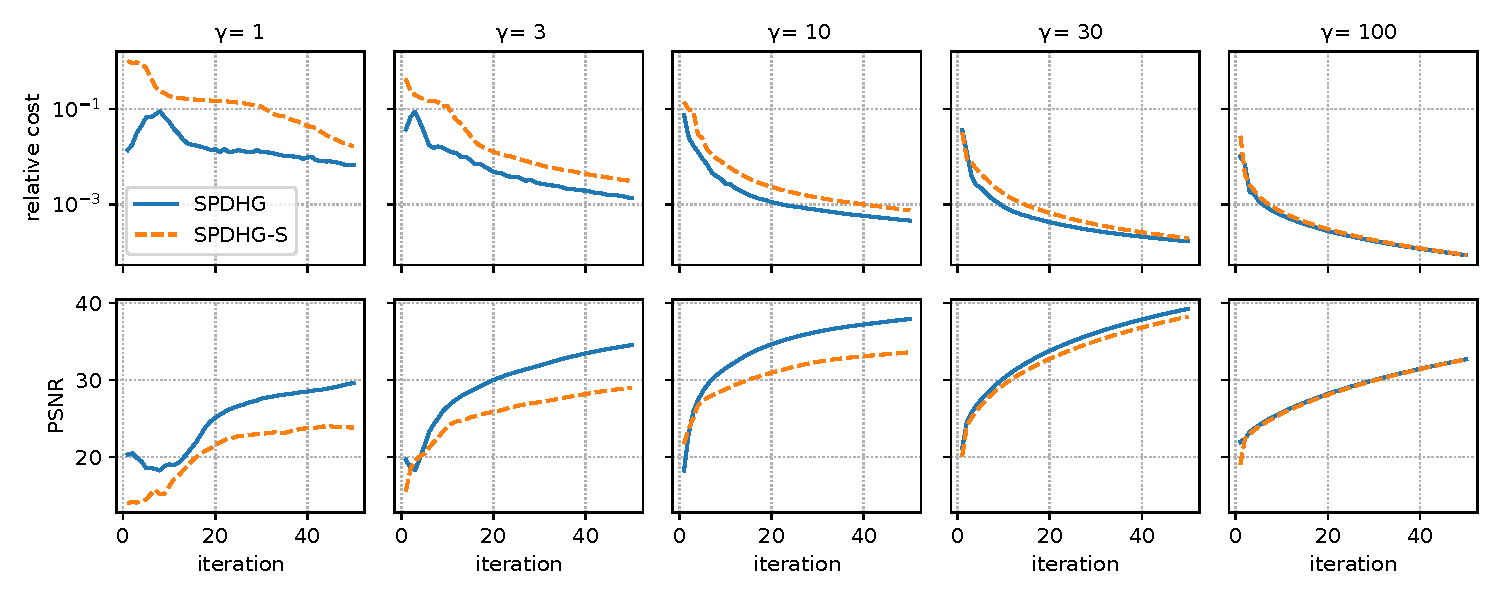
\includegraphics[width=1.0\textwidth]{./figs/fig1_brain2d_counts_1_0E+05_beta_6_0E-01_niter_5000_50_nsub_112_metrics.pdf}
  \caption{Cost and PSNR relative to the approximate minimizer of SPDHG and SPDHG-S for different
           $\gamma$ values, using $10^5$ counts and 112 subsets.}
  \label{fig:metrics}
\end{figure*}

\begin{figure*}
  \centering
  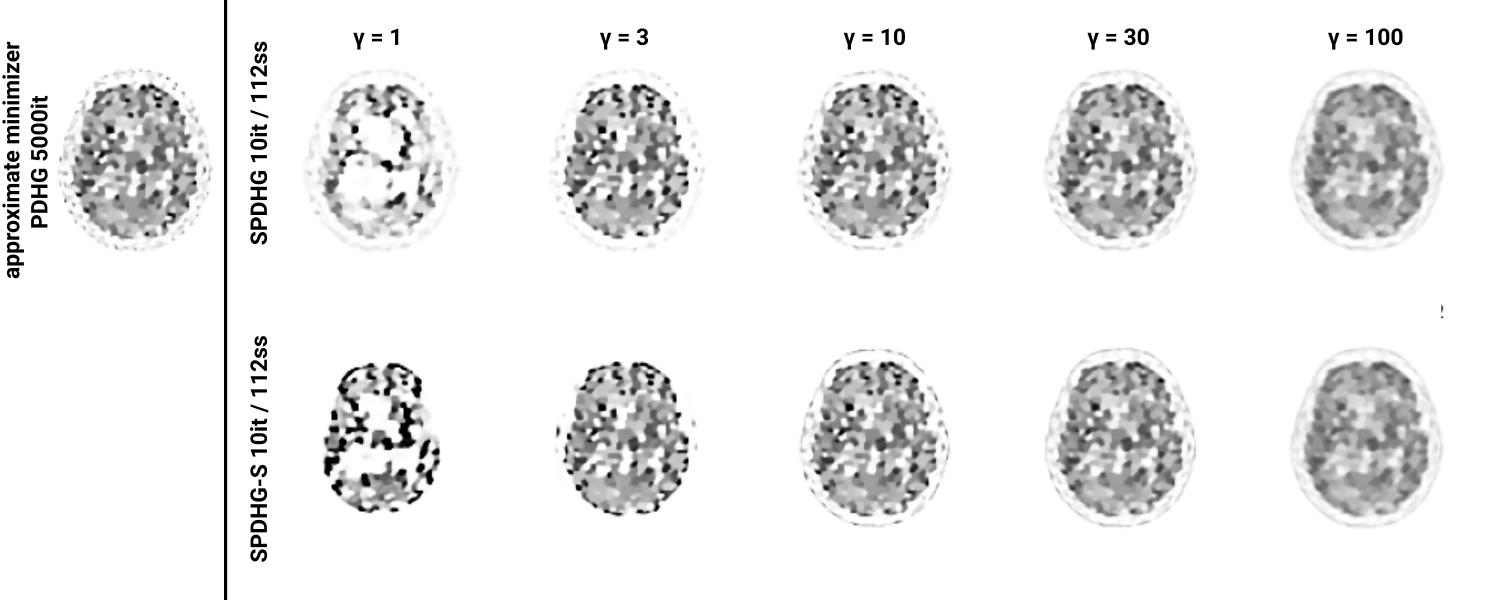
\includegraphics[width=1.0\textwidth]{./figs/fig2_recons_10_iterations.png}
  \caption{Reconstruction results of SPDHG (top) and SPDHG-S (bottom) after 10 iterations with
           112 subsets for different $\gamma$ values indicated above the reconstructions 
           using $10^5$ counts.}
  \label{fig:gamma}
\end{figure*}

\begin{figure*}
  \centering
  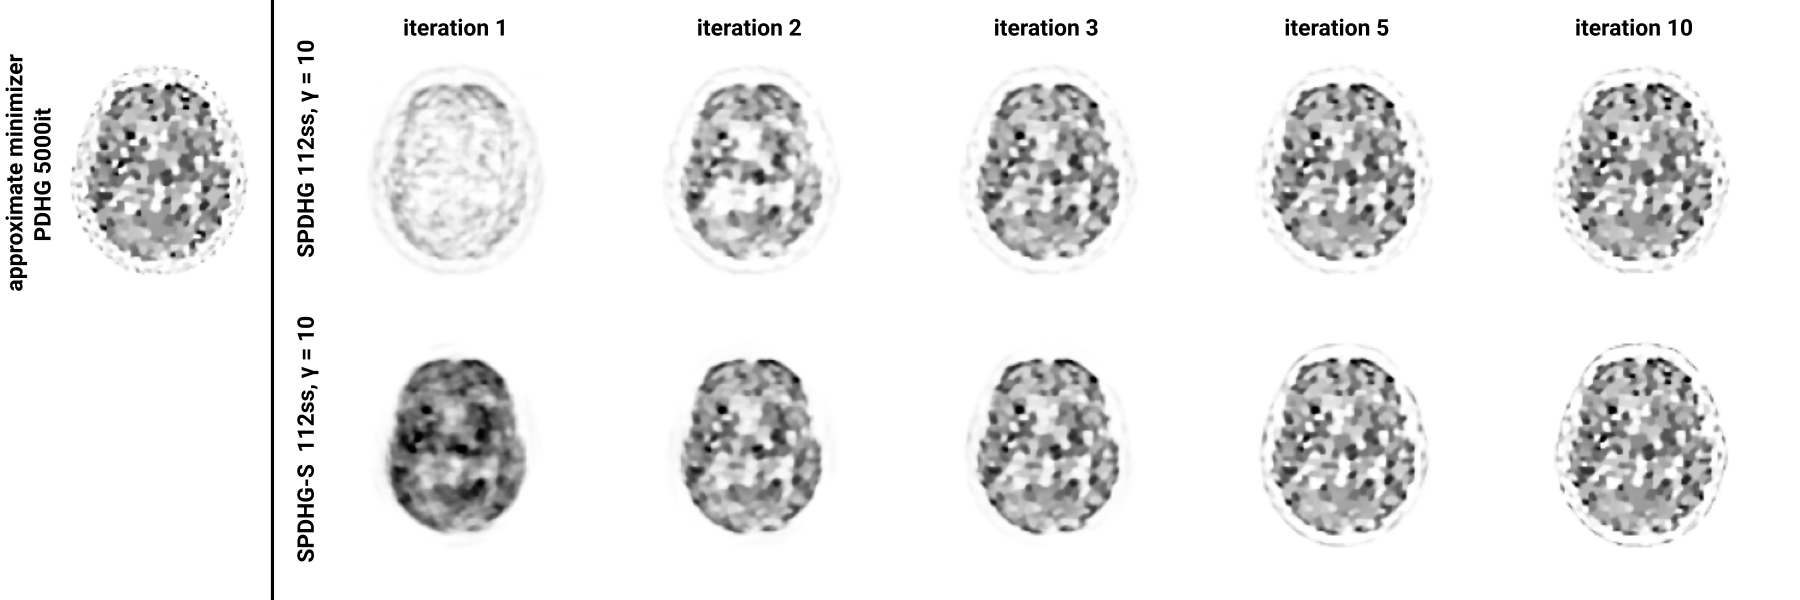
\includegraphics[width=1.0\textwidth]{./figs/fig3_early_iterations.png}
  \caption{Comparison of convergence of SPDHG (top) and SPDHG-S (bottom) in early iterations 
           using $10^5$ counts, $\gamma = 10$ and 112 subsets.}
  \label{fig:early}
\end{figure*}



\subsection{Numerical experiments}

To compare the convergence of SPDHG and SPDHG-S, we performed reconstructions of simulated
TOF PET data from a virtual 2D scanner mimicking the TOF resolution (ca. 400\,ps FWHM) and 
geometry of one ring (direct plane) of the GE SIGNA PET/MR (sinogram dimension: 
357 radial bins, 224 projection angles, 27 TOF bins).
A software brain phantom with a typical gray to white matter contrast of 4:1 was created
based on the brainweb phantom and used to generate simulated data including the effects
of attenuation and flat contamination (scattered) coincidences
with a simulated scatter fraction of 16\%.
Noisy simulated prompt emission TOF sinograms were generated for $10^5$, $10^6$, 
and $10^7$ counts. 
In the case of $10^5$, 80\% of the bins in the 2D TOF emission sinogram are 0.
The simulated data were reconstructed with SPDHG and SPDHG-S using 50 iterations, 112 subsets,
a fixed level regularization ($\beta = 0.6$ for $10^5$ counts, and $\beta = 0.2$ for $10^6$
and $10^7$ counts), and different values for $\gamma$.
As in \cite{Ehrhardt2019}, convergence was monitored by tracking the relative cost function
\[ c_\text{rel}(x) = (c(x) - c(x^*)) / (c(x^0) - c(x^*)). \]
and the peak signal to noise ratio 
\[ \text{PSNR}(x) = 20\,\log_{10} \left( \|x^*\|_\infty/\sqrt{\text{MSE}(x,x^*)} \right) \]
compared to an approximate minimizer $x^*$.
which was calculated using the deterministic PDHG with 5000 iterations without subsets.
In all reconstructions, the TOF PET operator $P$ was renormalized such that the norm of $P$
equaled the number of projection angles and the
subsets were defined via equidistant projection angles.
The gradient operator was implemented as the finite forward difference.


%-----------------------
%-----------------------
%-----------------------


\section{Results}

Figure~\ref{fig:metrics} shows the relative cost and PSNR to the approximate minimizer of 
SPDHG and SPDHG-S for different $\gamma$ values, using $10^5$ counts and 112 subsets.
First of all, we see that the choice of $\gamma$ has a strong influence on the convergence for
SPDHG and SPDHG-S which can be also seen in Fig.~\ref{fig:gamma} where the reconstructions
after 10 iterations are shown. 
Moreover, it can be observed in both figures that, 
with increasing $\gamma$, SPDHG-S performs more and more similar to SPDHG in terms 
of PSNR and the relative cost.
Figure~\ref{fig:early} shows a comparison of SPDHG and SPDHG-S in the very early iterations
for $\gamma = 10$.

\section{Discussion}

All three figures in this work demonstrate that the difference in the convergence between 
SPDHG and SPDHG-S for appropriate $\gamma$ values (e.g. 10) after ca. 3 iterations is very minor.
As reported in \cite{Ehrhardt2019}, we can confirm that after ca. 10 iterations the visual difference
in the image quality compared to the approximate minimizer is very small.
The remaining slight differences are mainly in low uptake regions in the skin around the brain.
Major differences in the convergence between SPDHG and SPDHG-S are only seen after the
1st iterations which is explained by the impact of the initialization of $y$ on the initialization
of $z$ and $\bar{z}$ as shown in line 2 in algorithm~\ref{alg:spdhg}.

The finding reported for $10^5$ counts were also confirmed for the higher count levels 
of $10^6$ and $10^7$ counts not shown here. 
However, note that at $10^7$ the emission sinogram is of less sparse
which naturally reduces the influence of our proposed initialization.
In contrast to \cite{Ehrhardt2019}, we find that in general $\gamma = 1$ is not optimal
in terms of convergence speed. 
Comparing the results with different simulated count levels, we find that the optimal value
for $\gamma$ is inversely proportional to the magnitude of the image to be reconstructed, or, 
in other words, inversely proportional to the number of acquired counts.

So far, the proposed SPDHG algorithm uses binned data (sinograms).
However, the promising results shown in this work might help to develop a convergent
algorithm that allows to directly reconstruct list-mode TOF PET data with non-smooth
priors.

\section{Conclusion}

The memory requirement for the SPDHG algorithm for sparse TOF PET data, can be
substantially reduced by a better initialization of the dual variable $y$ without
noticeable losses in the convergence speed.
Careful choice of the step size ratio parameter $\gamma$ depending on the magnitude
of the image to be reconstructed is crucial to obtain fast convergence.

%-------------------------------------------------------------------------------------------
\printbibliography

\end{document}
